\chapter[Introduction]{Introduction}\label{chap-intro}

%%%%%%%%%%%%%%%%%%%%%%%%%%%%%%%%%%%%%%
\section{Motivation and Background}
%%%%%%%%%%%%%%%%%%%%%%%%%%%%%%%%%%%%%%

The world’s population is projected to increase by nearly 2 billion in the next 30 years, of which 70\% will live in cities \citep{UNworldpop}. This growth is like adding an entire New York City to the planet every month \citep{unenvi2017}. In the face of increasing intensity and occurrence of hazards due to climate change (e.g. \citet{stewart2015, frangopol2020, IPCC_RN15}), urbanisation trends towards hazardous areas (e.g. \citet{mcgranahan2007rising,small2003global}), and rapid population growth, it is urgent to incorporate disaster risk reduction in accommodating these new citizens. This image of a riskier future may be bleak, but this presents a critical window of opportunity for the field of disaster risk management to tailor how and where to build this massive amount of new infrastructure that will lock us into a resilient trajectory for the next century.

Many cities already have an existing insurmountable risk, thus it is more practical to focus on mitigating future risk rather than existing risk. If we take Kathmandu, Nepal as an example, very little can be done to reduce the risk of the existing hundreds of thousands seismically-vulnerable buildings exposed to the region's high-seismic hazard. Displacement of a large amount of people to safer zones or rapid and massive-scale retrofitting are both impractical and infeasible. Thus, the best possible actions to reduce risk involve prioritising the management of future risk, and placing attention to critical infrastructure, which is something Nepal has started to do for schools \citep{dixit2014public}.

To guide such long-term proactive decisions for risk reduction, governments, international organisations, and the insurance industry rely on disaster risk analysis. For these actors, risk analysis serves as a powerful decision-making tool as it can quantify the likely damages, deaths, and losses from a potential hazard event, and highlight which risk reduction measures are most effective to reduce impact. By knowing and understanding the future impact of their policies, they can influence the distribution and quality of the future built environment in a way that is resilient.

The core procedure in disaster risk analysis is the convolution of hazard, exposure, and vulnerability, characterised in probabilistic terms. Thus, key to reliable disaster risk analysis is taking the best available representation of hazard, exposure, and vulnerability equipped with the best state-of-art methods that understand risk-sensitive forward planning.

It is encouraging that the past few decades have seen the development of state-of-art tools that help quantify risk from natural hazards (e.g. \citet{tralli2005satellite, liel2009incorporating, yun2015rapid, loos2020g}). Earthquake risk assessments, for instance, has greatly advanced in terms of predicting the probability of collapse of a building due to an earthquake in order to design mitigation strategies for a risk level acceptable for society (e.g. \citet{krawinkler2004performance,liel2006effectiveness, liel2008assessing, liel2012using}).  Yet despite the progress in our understanding of natural hazards and their impact, our current analysis tools fall short in their usability for decision makers who had to manage rapidly evolving and innovating cities. 

This PhD dissertation puts attention to three (3) broad issues that are currently under-emphasised in the development and implementation of current state-of-art analytics in risk and hazard quantification: (1) under-utilisation of advancements in hazard modelling using uncertain data, (2) lack of dynamic risk tools, and (3) lack of focus and ways to recognise successes from risk reduction measures. The first two issues were alluded in \cite{galasso2021risk}'s editorial that listed eleven (11) issues in current tools for decision support in risk reduction research and practice. The third issue was mentioned in \cite{lallemant2015modeling}'s concluding dissertation reflections about accountability of decision makers and the power of disaster risk models to enable recognition for sound decisions in risk. This dissertation does not cover other issues mentioned in \cite{galasso2021risk}, which include under-emphasis on social vulnerability, multi-hazard interaction, non-asset-based risk metrics, and involvement of users and local stakeholders. The purpose of this PhD dissertation is to develop new frameworks to shift the paradigm of current state-of-art analytics in risk and hazard quantification to better support decision-makers as they conduct risk-sensitive forward planning of the tremendous urban growth of the next few decades.

This chapter first defines key definitions in disaster risk analysis (Section \ref{subsec-int-def}) and presents three research gaps (\ref{subsec-int-gaps}). Three research questions that results from these gaps (presented in Section \ref{subsec-int-ques}) are each addressed in the main body of the thesis (Chapters \ref{chap-tephra}, \ref{chap-time}, and \ref{chap-counterfactual}). Section \ref{subsec-struct} briefly summarises key contributions and an overview of the dissertation structure.

% This chapter will provide an introduction to the study by first discussing the background and current challenges in analytics and support for regional scale risk reduction, followed by the dissertation's research questions and objectives. Lastly, an overview of the dissertation structure that highlights the contributions is provided.

%%%%%%%%%%%%%%%%%
\subsection{Definition of hazard, exposure, and vulnerability} \label{subsec-int-def}

Disasters are “social in nature” — they stem not solely from the hazard, but from the interactions of the physical, built, and social environments \citep{mileti1999disasters, peek2021interdisciplinary}. In turn, disaster risk can be broadly defined as the likelihood of future undesired consequences produced from potentially damaging events such as natural hazards as they interact with our built-natural-social environments. 

In this section, I define the core components in the quantification of disaster risk: hazard, exposure, and vulnerability. The convolution of these components can produce an estimate of the extent of a disaster, which can be characterised as loss of life, physical asset damage, and social, political and economic disruptions for a specific period of time \citep{smith2005through, moore1958tornadoes}. The quantification of disaster risk through the use of models and frameworks is critical in understanding potential disaster impacts for the design and evaluation of risk management strategies. Based on the terminology of \citet{assembly2016report}, hazard, exposure, and vulnerability can be defined as follows.

\begin{itemize}
    \item \textbf{Hazard} is defined as the likelihood of experiencing a certain intensity of potentially damaging event (e.g. earthquake, volcanic eruption, storm, etc.) at a certain location. The characteristics of hazards are typically identified by historical or user-defined scenario, probabilistic hazard assessment, and other methods that describe the hazard's location, intensity/magnitude, probability, and frequency.

    \item \textbf{Exposure} refers to the situation of built-natural-social environments located in zones affected by the hazard. Exposure may include people, infrastructure, housing, production capacities and socio-economic elements. Characterisation of exposure can be in terms of number of people or types of assets for the area and period of time of interest.

    \item \textbf{Vulnerability} refers to the susceptibility of the exposure to sustain impact or harm for a given hazard intensity. Vulnerability can be expressed as fragility or vulnerability functions that relate the expected level of damage or social cost (e.g. fatalities, displaced people) with the intensity of hazard, according to a specific exposure characteristic. The level of vulnerability can be influenced by physical, social, economic and environmental processes. Cultural and institutional factors have also been known to influence vulnerability such as poor design and construction of buildings, lack of awareness and risk communication, poverty levels and education, and disregard for responsible governance.
    
\end{itemize}

Some disaster risk frameworks include \textit{capacity} as an additional component to describe risk, where capacity is defined as the attributes, abilities, and resources available within a society to manage and reduce disaster risks and improve resilience \citet{assembly2016report}. Frameworks accounting for capacity are typically used for qualitative and index-based applications to analyse risk. As this dissertation focuses on quantitative frameworks to analyse risk, elements pertaining to capacity is not accounted for in the research.

In equation form, the impact resulting from a realised disaster event can be characterised in terms of its relevant risk parameters:

    \begin{equation}
    I_{realised} = f \left( \theta_H, \theta_E, \theta_V \right),
    \end{equation}

where $\theta_H$ are the hazard parameters (e.g. magnitude or intensity of the hazard occurrence), $\theta_E$ are the exposure parameters (e.g. location of buildings and number of people exposed), and $\theta_V$ are the vulnerability parameters (e.g. structural building characteristics, social vulnerability, etc.).

In most cases, a disaster event is considered as deterministic, assuming that all parameters $\theta_H, \theta_E, \theta_V$ are known and fixed. However, in some cases, some parameters are considered as fixed and others as unknown with known probability distributions, such as frequency-magnitude curves of earthquake occurrence. In such a scenario, the probability of each impact occurrence is linked to the probability of the unknown parameters. In practice, this type of calculation does not have an analytical solution and must be determined through simulation methods, such as Monte-Carlo simulation.

The case studies in this dissertation are limited to hazards caused by earthquake events and explosive volcanic eruptions. Specifically, the hazards of interest include ground shaking (disruptive up, down and sideways vibrations of the ground during an earthquake) and tephra fallout (fragments of rock ejected into the air by an erupting volcano that has the potential to form widespread deposits). Exposure elements in this thesis are buildings and people/occupants of the buildings exposed to the hazard.

The scope of this study is limited to the definition of vulnerability in the physical context only. Non-physical forms of vulnerability from damage caused by natural hazards such as social-vulnerability are not within the scope of this PhD dissertation. Thus, mentions of \textit{vulnerability} throughout the text is interchangeable with \textit{physical vulnerability}. Under this definition, examples of drivers that can increase physical vulnerability include deterioration processes such as corrosion, fatigue, creep, and hazard-induced damage. On the other hand, drivers that can decrease physical vulnerability are measures that adapt the infrastructure to future conditions such as retrofitting, maintenance, and building replacement and other strengthening interventions,

%% Include metric of impact
%% Define "long term DRR"
%% Hazards - What is dynamic hazard
%% Exposure - how it increases and decreases
%% Modeling urban change can take many forms (see sanderson paper for references)

%%%%%%%%%%%%%%%%%
\subsection{Current approach and challenges} \label{subsec-int-gaps}

This PhD dissertation addresses three challenges in analytics and support of regional scale risk reduction described below. The first two focuses on the \textit{analytics} aspect. These refer to challenges in the methodological features of our current risk analysis tools that limit their usability for decision makers amidst risk-sensitive forward planning for rapidly evolving regions. The third challenge focuses mostly on the \textit{support} aspect for decision-making in regional scale risk reduction. They refer to social-related factors that encourage and incentivise policy makers to promote greater resilience.

\subsubsection{Research gap 1}

\textbf{Hazard modelling rarely accounts for spatial characteristics and uncertainty in data} 

Modelling hazards phenomena often rely on the use of process-based models, which help represent the physical processes in the hazard. Two of the most useful applications of process-based models in hazard modelling are \textit{calibration/inversion} and \textit{forward estimation}. In inversion, hazard parameters that are often difficult or impossible to measure directly are estimated in such a way that they best represent the observed data. Common examples include estimation of earthquake rupture characteristics from seismic station records and calibration of volcanic eruption source parameters based on tephra deposit measurements (e.g. \citet{li2022comparative, georgoudas2007cellular, connor2006inversion}). In forward estimation, the calibrated hazard parameters are then used to estimate the response of the hazard system. For example, ground motion intensity can be estimated for a given earthquake rupture parameters \citep{worden2010revised, wang2022ground}. The accumulated tephra over a region can be estimated given eruption and wind parameters \citep{hurst1999performance, folch2009fall3d}. 

% This type of modelling is more commonly known as \textit{inversion modelling}, which often makes use of models that help represent the physical hazard phenomena, i.e. process-based models.
% calibration of floodplain characteristics based on historical flood events, 

% Modelling hazards phenomena rely on the estimation of hazard parameters that are often difficult or impossible to measure directly (e.g. earthquake rupture properties, total mass of ejected material from a volcanic eruption). Thus, to characterise the physical phenomena and processes in natural hazards analysis, models rely on the calibration of observed data. For instance, floodplain characteristics are calibrated based on observation of historical flood events, earthquake rupture characteristics are calibrated based on recordings at seismic stations, and volcanic eruption source parameters are based on measurements of the deposited tephra across the region of impact \citep{li2022comparative, georgoudas2007cellular, connor2006inversion}. This type of modelling is more commonly known as \textit{inversion modelling}, which often makes use of models that help represent the physical hazard phenomena, i.e. process-based models. The calibrated hazard parameters are then used to estimate the response of the hazard system. For example, given an inundation model and relevant floodplain parameters, locations of flooded areas on a map can be simulated \citep{uhlenbrook2004hydrological}. Ground motion intensity can be estimated for a given earthquake rupture parameters \citep{worden2010revised, wang2022ground}. The accumulated tephra over a region can be estimated given eruption and wind parameters \citep{hurst1999performance, folch2009fall3d}. This type of modelling is referred to as \textit{forward modelling}.

As hazard models consider more complex processes, and as multiple data sources are increasingly becoming more available (e.g. ground sensors, crowd-sourcing, and remote sensing), current inversion and forward estimation frameworks ignore particular characteristics in the data that they rely on (e.g. spatial properties, distribution, and uncertainty \citep{willcox2021imperative}. Not accounting for these characteristics in the data may result to significant bias in the model outputs, and influencing their predictive performance in an extent that is currently under-explored. 

In Chapter \ref{chap-tephra}, these issues are explored in the context of modelling tephra fallout from explosive volcanic eruptions. The spatial and uncertainty characteristics in both the model calibration (inversion) phase and forward estimation phase are studied to improve the estimated parameters and model outputs. Given that tephra measurements are often collected in batches by different fieldwork teams at different durations since the eruptive event, there is value in accounting for uncertainty variations and spatial properties in the data. Measurements that are most reliable and contain the least uncertainty are mostly those taken from a well-preserved deposit, i.e. those taken soon after an eruption has ended in areas with little deposit reworking by wind and surface runoff processes \citep{PYLE201625, blong2017}. The study addresses the current lack of conventional approaches in tephra fall modelling to consider differential uncertainties, and spatial nature in data for both calibration and forward estimation settings.


\subsubsection{Research gap 2}
    
\textbf{Current risk analysis methods are not future-focused; they represent static vulnerability and exposure} 
% Use QE slide materials if i decide to use graphical abstracts

Current risk analysis methods were not developed to account for future risk -- they quantify disaster risk in the context of present day's built environment, and are developed to represent static vulnerability and exposure. In a literature review by \citet{newman2017review} of more than 100 risk analysis methods for decision making, 78\% consider a short-term perspective, which are typically catered towards the insurance perspective (3 to 5-year time horizon). While many of such modeling and simulation tools provide useful scenarios and cost-benefit evaluations for natural hazard mitigation plans (e.g. \citet{mostafavi2021toward, nofal2021high, talebiyan2018risk, wang2020computational}), their static nature will underestimate risk and limit proactive decisions to reduce future risk. The remaining 22\% studied by \citet{newman2017review} with a long-term perspective (30+ years) account for future risk only in terms of changing hazards (i.e. changing climate). The future-focused models in \citet{newman2017review}'s review only accounts for the current condition of the infrastructure. Not only the impact of climate change on natural hazards, but also population growth, economic development and changing vulnerabilities are significant long term drivers for risk that should be accounted for within risk reduction planning and risk modelling. On a positive note, there has been a recent shift in the field of disaster resilience towards a more dynamic and future-focused lens (e.g. \citet{cremen2021modelling, galasso2021risk, hemmati2020role, sanderson2022coupled}) indicating that the discipline of dynamic risk quantification is a rapidly growing field.

Studies about dynamic exposure have demonstrated many approaches to model changes in the urban footprint such as cellular automata methods \citep{chaudhuri2013sleuth, white1993fractal} and agent-based modeling \citep{huang2014review, parker2008conceptual}. In addition, several studies have been combining such urban change dynamic models with hazard consequence models to calculate regional risk. Recent studies include \citet{deierlein2021state, mesta2022urban, williams2022regional, calderon2021exposure, cremen2022simulation, hemmati2021shaping, sarica2020spatio, haer2020safe}, .

Meanwhile, time-dependent vulnerability for risk analysis has been studied in the context of single buildings and infrastructure. One exception is \citet{lallemant2017framework}'s study where a time-dependent vulnerability framework was used to provide projections of building collapse for a neighborhood-scale in Kathmandu Valley, Nepal. \citep{lallemant2017framework}'s work considered incremental building expansion as the driver of changing vulnerability. Incremental building expansion is a common informal construction practice for developing countries around the world to respond to growing housing needs, which often involves adding one or multiple floors to houses \citep{amoako2017build, ferguson2010finance}.

The single-building applications for time-dependent vulnerability are in the context of seismic aftershock damage, deterioration, corrosion, and climate change adaptation. Examples of studies that assessed \textit{increasing} vulnerability in terms of damage accumulation to buildings due to an earthquake aftershock sequence include \cite{raghunandan2015aftershock, aljawhari2021effects, gentile2021hysteretic, papadopoulos2021exploring}. Research on environment-induced deterioration (e.g. corrosion) as it changes the physical vulnerability of the built environment has also been advancing in recent years to cover different components of buildings and bridges \citep{kashani2019residual, amaya2019reliability, guo2019critical, zanini2020seismic, rao2017development, zamanian2020high} and to account future weather conditions \citep{bastidas2015damage, bastidas2016economic, wang2012impact, stewart2012climate, el2010reliability, yang2019societal, sevieri2021typhoon}. Studies have also assessed \textit{decreasing vulnerability} as achieved by adaptation measures to infrastructure to future conditions. Many of such studies are motivated by climate adaptation strategies to reduce vulnerability against wind and flood-induced damage (e.g. \citet{stewart2014climate, dong2017adaptation, li2011cyclone, qin2020risk,ward2017global}). 

Based on the studies mentioned, current risk analysis methods are not future-focused, with time-dependent vulnerability modelling being the most limited in terms of regional-scale applications. In addition studies on dynamic vulnerability focus only on one driver of changing vulnerability for each application at a time. Currently, there is still no conventional framework to simultaneously model multiple drivers that may increase and/or decrease physical vulnerability of exposed structures. As regions may experience these multiple drivers at the same time, accounting for them is critical to properly understand hazard-related risk over the lifespan of the built environment. Chapter 3 explores these research gaps in the context of earthquake risk modelling.


\subsubsection{Research gap 3}

\textbf{Successes in risk reduction measures are often invisible, resulting to lack of incentives to proactive decision-making.}

    Disaster risk reduction efforts try to ensure that losses from disaster are avoided (i.e. `nothing happens'). However, this poses a dilemma for recognising and incentivising successful risk interventions since they are made \text{invisible} by the very nature of their success. As a result, there is often a lack of incentives for decision makers to commit and invest in disaster risk reduction.

    One situation where effective risk reduction is made invisible occurs when success has not been realised because the hazard has not occurred. If the benefits of risk reduction actions manifest primarily as reduced impact when a hazard event occurs, these benefits may only be realised far in the future — particularly for rare and extreme events. Hence relying on the realisation (also known as outcome bias) of a disaster to evaluate mitigation efforts ignores the significant time delay between the investment in risk reduction and the hazard. As with many actions to mitigate climate change, disaster risk reduction interventions require immediate sacrifice for seemingly uncertain benefits at a much later time \citep{weber_experience-based_2006}. This time delay means that risk mitigation successes are rendered invisible until the eventual realisation of a hazard; excepting situations when mitigation measures also introduce co-benefits, in which risk reduction investment not only mitigates risk but also fosters economic growth or other societal welfare \citep{Tanner2015}.

    Another situation where success in risk reduction becomes invisible is when a large hazard event occurs with disastrous impacts to society. In midst of the loss of life and negative societal and economic impacts from the disaster, both news and research tend to focus on the catastrophe. For this situations, it is very rare that a past mitigation intervention is revisited for analysis to assess how effective it was. This invisibility of mitigation successes amidst catastrophe is exacerbated by the perception that disasters are rare, overwhelming “acts of god” for which it is impossible to prepare \citep{gaillard_disaster_2019}. 

    The field of social psychology provides further insight into why disaster risk reduction evaluation is often so challenging based on the concepts of risk perception. Research has shown that people’s emotional responses to events are influenced by their perception of ``what might have been" \citep{medvec_when_1995,roese_what_2014}. A disaster event is a break from normalcy that triggers imaginations of alternative realities or \textit{counterfactuals}: What if the disaster had never happened? What if it had hit a neighbouring town instead? In the aftermath of negative experiences, these counterfactuals are usually in an “upward” direction, where one imagines a better outcome than the realised outcome \citep{blix_thinking_2016}, e.g. thinking about the ways in which a past car accident could have been avoided. Perceiving the benefits of mitigation, however, often requires comparing reality to a worse outcome or ``downward counterfactual", which is not a natural cognitive process, e.g. imagining how a past car accident could have been worse. 
   
    Driven by these challenges related to risk perception and outcome bias, four types of situations arise wherein successful disaster risk reduction interventions are made invisible. Each of these situations can be visualised with a simple graphic using stilt houses as the mitigation and flooding as the hazard shown in Figure \ref{fig:motivation}.
    
    \begin{enumerate}
    \item \textbf{Success made invisible in the midst of broader disaster:} Successful mitigation may result in fewer losses after a disaster, but this success is obscured amid the catastrophe and losses that were still incurred.
    
    \item \textbf{Success made invisible by nature of the success:} A hazard becomes a disaster on account of the impacts it has on society. If mitigation efforts are so successful that there are no perceivable impacts, both the potential disaster and the successful mitigation are made invisible.
    
    \item \textbf{Success made invisible due to yet unrealised benefits:} On account of the large time delay between the mitigation intervention and its benefits being realised, mitigation efforts could be seen as unsuccessful or unnecessary until a hazard event occurs.
    
    \item \textbf{Success made invisible by the randomness of the specific outcome:} hazards are stochastic processes, hence any single occurrence is only one of several possibilities that could have occurred. Recognising that the parameters of the event that actually occurred could easily have been different, successes can be made invisible if the hazard randomly does not strain mitigation measures, e.g. a near-miss.   
    \end{enumerate}

     %% Figure of types of invisibility
    \begin{figure}[h!]
    \begin{center}
     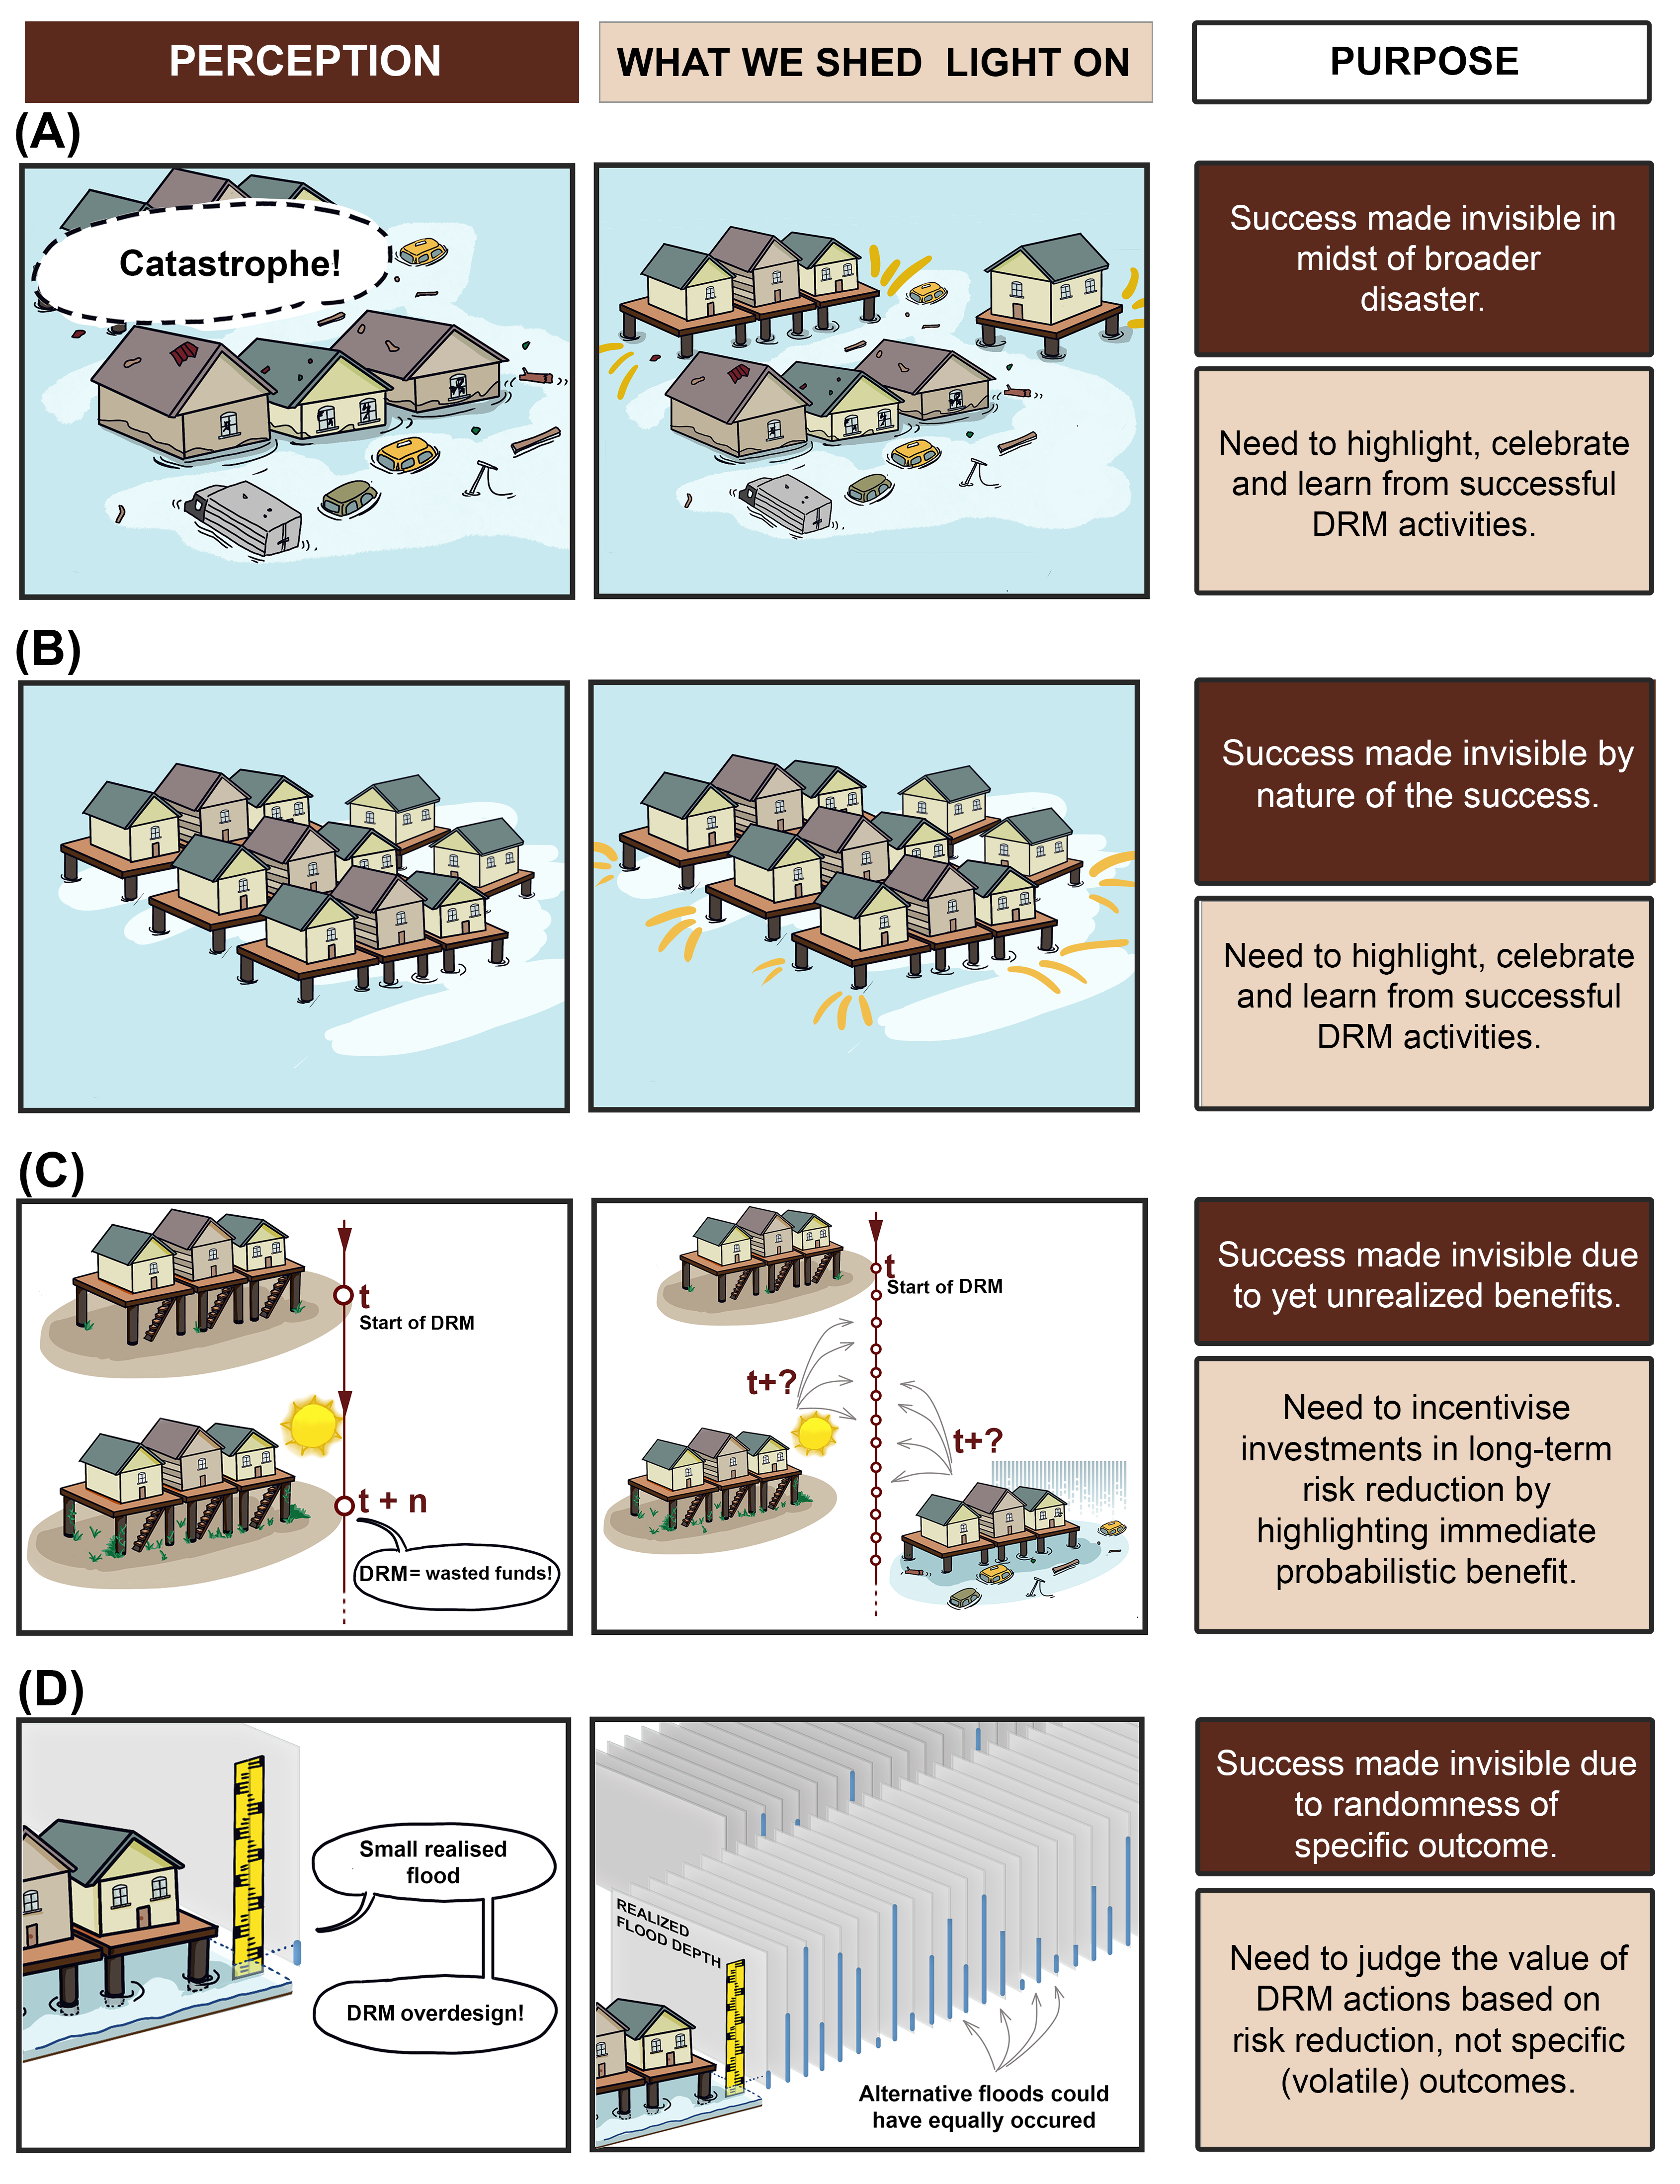
\includegraphics[width=\linewidth]{Figures/fig1_motivation.png}
		\caption{A schematic of invisibilities in mitigation successes using stilt houses as the mitigation and flooding as the hazard. This figure was developed and presented in published report for the 2022 Global Assessment Report, which I lead \citep{lallemant_rabonza_gar_2022}. Chapter \ref{chap-counterfactual} aims to address the first and the third invisibility described in this figure: (a) success invisible in midst of broader disaster, and (b) success made invisible due to yet unrealised benefits.}
	\label{fig:motivation}
	\end{center}
    \end{figure}

    Investing in disaster mitigation is essential, particularly with the rising frequency of disasters due to climate change \citep{IPCC_RN15}. However, doing so in the light of the time delay between taking action and seeing benefits, as well as the invisibility of successful risk reduction, means that decisions to invest in mitigation require remarkable political will. Without recognition and reward for these efforts, interventions may be perceived as ineffective or unnecessary, with potentially disastrous consequences. Thus, highlighting the invisible benefits of successful risk reduction is critical, as celebrating past successes can help sustain and amplify ongoing efforts, and provide positive examples to learn from, rather than focusing only on negative events that often dominate the news and research \citep[e.g.][]{leach2012transforming, scott1998seeing}.

    How then can policymakers be incentivised to make better risk-informed decisions when they are not credited for pro-active actions nor accountable for the consequences of doing nothing? There is a pressing need to develop better frameworks to judge the successes of disaster risk reduction interventions, both to recognise and celebrate good decisions as well as to create incentives for further investment in mitigation.
    
    Chapter 4 addresses this research gap in the context of earthquake risk modelling. Specifically, the chapter covers analytics that address two out of the four situations of invisibility in disaster risk reduction: success made invisible in the midst of broader disaster, and success made invisible due to yet unrealised benefits (represented in Figures \ref{fig:motivation}A and \ref{fig:motivation}C).

%% Currently, there is a stronger incentive to post-disaster response than preparation. 
%% See TAC 2020 - write up on outcome bias using Haiti and Sendai Framework references

%%%%%%%%%%%%%%%%%%%%%%%%%%%%%%%%%%
\section{Research questions} \label{subsec-int-ques}
%%%%%%%%%%%%%%%%%%%%%%%%%%%%%%%%%%

The main focus of this dissertation has been to develop new frameworks to shift the paradigm of current state-of-art analytics in risk and hazard quantification towards better support tools for decision-making to reduce risk of highly dynamic regions. This aim considers that current state-of-art frameworks would provide more value for decision-makers in risk reduction when they (1) consider spatial and uncertainty characteristics in the data, (2) account for the dynamic changes in the built environment, (3) provide incentives or credit to implement proactive risk reduction measures.
% The process to develop these frameworks require research on state-of art analytics in hazard prediction, vulnerability modelling, urban change dynamics, and risk perception. Researching these topics for different types of hazard applications shed light on limitations and challenges in the current approaches in terms of their usability to create proactive decisions for risk reduction. 

The specific research questions of the dissertation are:

\begin{enumerate}
    \item How can we make the most of limited and uncertain spatial data in inversion and forward estimation with process-based hazard models? 

    \item How do we account for time-dependent physical vulnerability in regional scale seismic risk analysis?

    \item How do we highlight the success of risk reduction programs implemented in the past and the benefits they will provide in the future using risk analytics?
\end{enumerate}

%%%%%%%%%%%%%%%%%%%%%%%%%%%%%%%%%%
\section{Summary of contributions and structure} \label{subsec-struct}
%%%%%%%%%%%%%%%%%%%%%%%%%%%%%%%%%%

% The organisation of the PhD dissertation is shown in Figure XX. 
The body of this  dissertation is a collection of three papers, corresponding to Chapters \ref{chap-tephra} through \ref{chap-counterfactual}. Chapters \ref{chap-tephra} and \ref{chap-time} introduce improved risk \textit{analytics} that enable risk-sensitive forward planning in regions where the built environment is rapidly evolving. Chapter \ref{chap-counterfactual} focuses on the \textit{support} aspect for decision-making in regional scale risk reduction. The chapters address the research questions in the context of earthquake and volcano hazards. Each chapter is autonomous with its own introduction and conclusion. References for all chapters are compiled at the end. 

Contributions of the research project are summarised briefly below, and described in detail in each chapter. Their significance are discussed in the concluding chapter. The contributions all fit together to contribute to the vision of the PhD research: to provide evidence and tools for promoting greater resilience. 

%%%% Set colors to list of Contributions
\newcommand{\varitem}[3][black]{%
  \item[ \colorbox{#2}{\textcolor{#1}{\makebox(5.5,7){#3}}}  ]}

\vspace{1cm}
\noindent
\textbf{Chapter 2: Inversion and forward estimation with process-based hazard models: an investigation into cost functions, uncertainty-based weights and model-data fusion}
\noindent

Chapter \ref{chap-tephra} investigates methods that account for spatial-dependence and uncertainty in hazard modelling using limited and uncertain spatial data. Using an example of reconstructing past volcanic eruption characteristics and associated tephra fallout from different sets of field observation, I demonstrate the importance of making the best use of data-related uncertainty and spatial information in inversion and forward estimation. I present strategies for: (1) the selection of appropriate cost functions for inversion / calibration of a hazard model, accounting for their behaviour and the implied distribution of residuals, (2) the treatment of differential uncertainty when combining multiple data, and (3) the leveraging of both model and data when estimating the spatial distribution of output. These are demonstrated using data from the tephra fallout of the 2014 eruption of Kelud volcano in Java, Indonesia, and the Tephra2 model (a state-of-art approach in modelling the tephra fall accumulation around the regional vicinity of a volcano after an explosive eruption). This study makes use of methods in tephra fall hazard modelling, spatial statistics, goodness-of-fit tests, and calibration of models. Chapter \ref{chap-tephra}'s specific contributions include:

\begin{enumerate}

\varitem{orange!40}{\textbf{a)}} 
Proposed a two-step approach to evaluate the choice of cost function for inversion/calibration problems using process-based models.

\varitem{orange!40}{\textbf{b)}}
Demonstrated that the impact of the choice of cost function in inversion is significant. This is the first study to place attention and investigate these impacts for tephra fall inversion.

\varitem{orange!40}{\textbf{c)}}
The study added three more alternative cost functions to the default Tephra2 code, and identified one that is best-suited for the case study.

\varitem{orange!40}{\textbf{d)}}
Extended the Tephra2 inversion algorithm to account for varying uncertainty across different data points, rather than treating each data point equally in the optimisation.

\varitem{orange!40}{\textbf{e)}}
Developed a model-data fusion approach based on spatial statistics methods that combines the forward model output and the data to improve estimates of the spatial distribution of tephra fall load. 

\varitem{orange!40}{\textbf{f)}}
Extended the model-data fusion methodology to also account for different levels of uncertainty associated with different sets of data. 

\varitem{orange!40}{\textbf{g)}}
Produced not only a map of tephra distribution, but also a map of uncertainties associated to the modelled tephra load in a forward estimation. 


\end{enumerate}



\vspace{1cm}
\noindent
\textbf{Chapter 3: Regional scale risk analysis accounting for time-dependent vulnerability}
\noindent

Chapter \ref{chap-time} presents a flexible framework to account for time-dependence in physical vulnerability for seismic risk analysis. Processes that increase vulnerability and policies that mitigate increase in vulnerability are modeled  using time-homogenous Markov chains. The various state change processes are integrated within the risk analysis framework in closed form expressions. A hypothetical building stock with fragility curves derived from literature are utilised to demonstrate the framework. Multiple applications are demonstrated: (1) quantifying risk of structurally deteriorating buildings and the risk reduction impact of maintenance, (2) urban-scale seismic retrofitting policies based on various retrofit rates, and (3) impact of varying rates of building replacement to higher design grade, and an application wherein several drivers of changing vulnerability were implemented in the analysis. Chapter \ref{chap-time}'s specific contributions are:

\begin{enumerate}
\varitem{orange!40}{\textbf{a)}} 
Extended the Performance-Based Earthquake Engineering (PBEE) methodology \citep{krawinkler2004performance} framework (the state-of-art engineering approach to assess impact from earthquake damage) to incorporate time-dependent vulnerability driven by multiple regional scale policies and deterioration. 

\varitem{orange!40}{\textbf{b)}} 
Proposed to integrate a Markov chain approach with the risk analysis framework to model future regional-scale seismic risk driven by time-dependent vulnerability

\varitem{orange!40}{\textbf{c)}} 
Demonstrate through case studies the influence of time-dependent vulnerability on a single deteriorating building, and to a neighborhood with buildings experiencing deterioration, retrofitting, and building replacements over time.

\varitem{orange!40}{\textbf{d)}} 
Introduced a proof of concept and flexible tool for decision-makers to investigate the consequences of various seismic mitigation decisions (that influence physical vulnerability) to future seismic risk. 


\end{enumerate}


\vspace{1cm}
\noindent
\textbf{Chapter 4: Learning from successes, not catastrophe: Using counterfactual analysis to highlight successful disaster risk reduction intervention}
\noindent

In Chapter \ref{chap-counterfactual}, a framework is proposed for incentivising risk-informed measures by estimating the benefits of an intervention in a past earthquake, and for a hazard that has not yet occurred. The approach uses counterfactual modelling of a past hazard event with consequences made worse (i.e. downward counterfactual) by the absence of the mitigation intervention. Using a school building database for Kathmandu Valley, Nepal, two applications are presented: (1) the quantification of lives saved during the 2015 Gorkha earthquake as a result of the retrofitting of schools in Kathmandu Valley since 1999, (2) the quantification of the annual expected lives saved if the pilot retrofitting program was extended to all school buildings in Kathmandu Valley based on a probabilistic seismic hazard model. The analyses highlights the success of the seismic retrofitting program for schools in Nepal during the Gorkha earthquake, and the benefits of scaling up the program. Chapter \ref{chap-counterfactual}'s specific contributions are:

\begin{enumerate}
\varitem{orange!40}{\textbf{a)}} 
Introduced conceptual situations where successful disaster risk management interventions are made invisible with discussion derived from risk perception and social psychology.

\varitem{orange!40}{\textbf{b)}} 
Proposed a framework to quantify and highlight the benefits of effective disaster risk reduction interventions for two situations where they go unnoticed: amidst disaster, and when benefits are not yet realised by a hazard occurrence.
% Proposed a framework to quantify and highlight lives saved from effective disaster risk reduction interventions, that otherwise go unnoticed. The framework is a combination of the traditional probabilistic risk analysis framework and counterfactual analysis. By using an appropriate counterfactual scenario as a baseline against which to compare realised outcomes, the framework makes clear that the impact of hazards would be much worse without important investments in risk reduction.

\varitem{orange!40}{\textbf{c)}} 
Introduced a new domain of application for counterfactual analysis in disaster research: highlighting the positives in disaster mitigation. Previous applications focus on identifying worse disaster outcomes for the purpose of insurance, preparedness, or future mitigation.
% The study uses downward counterfactual risk analysis to provide analytical evidence of the benefits of effective risk reduction.

\varitem{orange!40}{\textbf{d)}} 
Pioneered a systematic approach to create incentives for good decision-making in risk reduction through quantification of probabilistic lives saved.
% The study pioneered a systematic approach to create incentives for good decision-making on the basis of probabilistic risk. The quantification of probabilistic lives saved by effective risk reduction programs in a major hazard event serves as a powerful indicator of the intervention’s success that would otherwise remain unnoticed amidst a disaster. In addition, the calculated probabilistic benefits of an intervention provide important incentive and encouragement to decision-makers committed to implementing effective measures even if the benefits are not materialized yet by the occurrence of a hazard event.

\varitem{orange!40}{\textbf{e)}} 
Compiled a list of other potential applications of the proposed framework beyond earthquake risk reduction and retrofitting program for schools.
% Compiled a list of other potential applications of the proposed framework beyond earthquake risk reduction and school retrofitting programs. A table of examples were provided that covers various natural hazard applications, as well as intervention types that could be celebrated using counterfactual analysis.

\end{enumerate}

Chapter \ref{chap-conc} concludes the dissertation by summarising and synthesising the contributions of the research. The limitations and future recommendations for research are also presented.

Every chapter is introduced with three to four bullet points that serve as my "elevator pitch" for the chapter. They capture key methods and results presented in the chapter, but don't necessarily include all ideas, concepts or conclusions. Notational convention may not be strictly consistent across chapters, since notation was chosen for each paper rather than for the entire dissertation. Appendices for each chapter are compiled and organised at the end of the dissertation. This dissertation is a non-exhaustive representation of the work and research that I have conducted at Nanyang Technological University in the past 4.5 years.
